\documentclass[]{tufte-book}

% ams
\usepackage{amssymb,amsmath}

\usepackage{ifxetex,ifluatex}
\usepackage{fixltx2e} % provides \textsubscript
\ifnum 0\ifxetex 1\fi\ifluatex 1\fi=0 % if pdftex
  \usepackage[T1]{fontenc}
  \usepackage[utf8]{inputenc}
\else % if luatex or xelatex
  \makeatletter
  \@ifpackageloaded{fontspec}{}{\usepackage{fontspec}}
  \makeatother
  \defaultfontfeatures{Ligatures=TeX,Scale=MatchLowercase}
  \makeatletter
  \@ifpackageloaded{soul}{
     \renewcommand\allcapsspacing[1]{{\addfontfeature{LetterSpace=15}#1}}
     \renewcommand\smallcapsspacing[1]{{\addfontfeature{LetterSpace=10}#1}}
   }{}
  \makeatother

\fi

% graphix
\usepackage{graphicx}
\setkeys{Gin}{width=\linewidth,totalheight=\textheight,keepaspectratio}

% booktabs
\usepackage{booktabs}

% url
\usepackage{url}

% hyperref
\usepackage{hyperref}

% units.
\usepackage{units}


\setcounter{secnumdepth}{-1}

% citations
\usepackage{natbib}
\bibliographystyle{plainnat}


% pandoc syntax highlighting

% longtable

% multiplecol
\usepackage{multicol}

% strikeout
\usepackage[normalem]{ulem}

% morefloats
\usepackage{morefloats}


% tightlist macro required by pandoc >= 1.14
\providecommand{\tightlist}{%
  \setlength{\itemsep}{0pt}\setlength{\parskip}{0pt}}

% title / author / date
\title[Selection Criteria]{SIVOCS Interview Candidates \textbar{} Batch
2}
\date{2021-12-21}


\begin{document}

\maketitle




\hypertarget{selection}{%
\chapter{Selection}\label{selection}}

The second batch of interview candidates focuses on unusual or
unexpected cases along with the projects that scored high in one or
multiple SI-related variables. There are 2 main clusters that
encapsulate the selection process; Cluster 1 is generally concerned with
the projects that have been relatively high rated regarding multiple
outcome variables despite having low ratings in other key SI variables
or vice versa and Cluster 3 includes the projects that have overall high
rating in key SI variables.

The criteria used for each cluster is as follows.

\hypertarget{cluster-1-19-projects}{%
\section{Cluster 1 (19 projects):}\label{cluster-1-19-projects}}

\begin{itemize}
\tightlist
\item
  Low motivation to benefit society - High SI contribution
  (self-assessment)
\item
  Low transdisciplinary involvement - High public outcome
\item
  Low motivation to improve human condition - high impact statement on
  emancipation/ capability/ understanding
\end{itemize}

\hypertarget{cluster-3-12-projects}{%
\section{Cluster 3 (12 projects):}\label{cluster-3-12-projects}}

\begin{itemize}
\tightlist
\item
  High motivation to imp. human condition + changed behaviour (public,
  policy, civil society orgs)
\item
  High SI familiarity (and/or high overall SI stats)
\end{itemize}

\hypertarget{final}{%
\section{Final}\label{final}}

After a manual elimination, from the \textasciitilde80 selected
projects, approximately 38 relatively less related projects are
eliminated, \textbf{leaving 42 respondents in total} (12f \textbar{} 29
\textasciitilde{} 30\%).

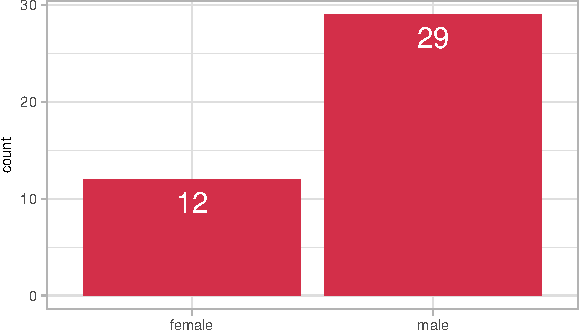
\includegraphics{15_interview_cand_2_files/figure-latex/gender-1}

Also, the distribution of the sci. domains in the final sample is as
follows:

\begin{figure*}
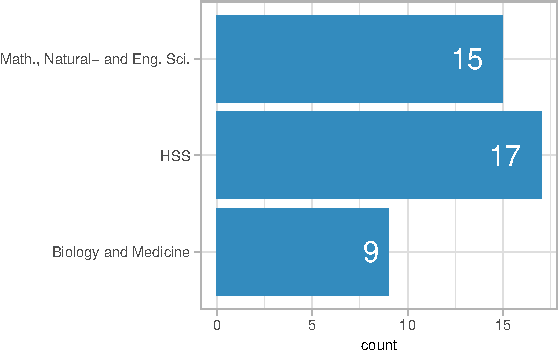
\includegraphics{15_interview_cand_2_files/figure-latex/unnamed-chunk-2-1} \end{figure*}

\bibliography{skeleton.bib}



\end{document}
